\documentclass[12pt]{article}
\usepackage[utf8]{inputenc}
\usepackage{float}
\usepackage{amsmath}


\usepackage[hmargin=3cm,vmargin=6.0cm]{geometry}
%\topmargin=0cm
\topmargin=-2cm
\addtolength{\textheight}{6.5cm}
\addtolength{\textwidth}{2.0cm}
%\setlength{\leftmargin}{-5cm}
\setlength{\oddsidemargin}{0.0cm}
\setlength{\evensidemargin}{0.0cm}

%misc libraries goes here
\usepackage{tikz}
\usepackage{amssymb}
\usetikzlibrary{automata,positioning}

\def\firstcircle{(0,0) circle (1.5cm)}
\def\secondcircle{(0:2cm) circle (1.5cm)}

\colorlet{circle edge}{blue!50}
\colorlet{circle area}{blue!20}

\tikzset{filled/.style={fill=circle area, draw=circle edge, thick},
    outline/.style={draw=circle edge, thick}}

\setlength{\parskip}{5mm}

\begin{document}

\section*{Student Information } 
%Write your full name and id number between the colon and newline
%Put one empty space character after colon and before newline
Full Name : Yavuz Selim Yesilyurt \\
Id Number : 2259166 \\

% Write your answers below the section tags
\section*{Answer 1}

\subsection*{a.}
\hspace{6mm}	
Let us denote every number that the set of rational numbers inside the open interval $(-1,0)$ contains $n$ as $n = \frac{a}{b}.$ We can write the elements of this set as;
\begin{center}
\begin{tabular}{ c| c c c c c}
 $a \setminus b$  &$ 1$ & $2$ & $3$ & $4$ & ...  \\
   \hline
 $ -1$ & $-\frac{1}{1}$ & $-\frac{1}{2}$ & $-\frac{1}{3}$ & $-\frac{1}{4}$ & ...\\
 $ -2$ & $-\frac{2}{1}$ & $-\frac{2}{2}$ & $-\frac{2}{3}$ & $-\frac{2}{4}$ & ...\\
 $ -3$ & $-\frac{3}{1}$ & $-\frac{3}{2}$ & $-\frac{3}{3}$ & $-\frac{3}{4}$ & ...\\
 $ -4$ & $-\frac{4}{1}$ & $-\frac{4}{2}$ & $-\frac{4}{3}$ & $-\frac{4}{4}$ & ...\\
 ... & ... & ... & ... & ... & ...\\
\end{tabular}
\end{center}

In table, first row, above the horizontal line contains the countably infinite elements of set $\mathbb{N}$ except $0$, starting from 1 and the first column, left of vertical line contains the countably infinite elements of set $Z^-$ except $0$. The entries in the upper half (triangular) of this table (above the diagonal, diagonal is exclusive) illustrates the numbers $n = \frac{a}{b}$ that is in this set. They can be counted reverse diagonally starting with $-\frac{1}{2}$ (i.e. 1st element: $-\frac{1}{2}$, 2nd element: $-\frac{1}{3}$, 3rd element $-\frac{2}{3}$, 4th element: $-\frac{1}{4}$, 5th element: $-\frac{1}{5}$, 6th element: $-\frac{2}{4}$, 7th element: $-\frac{3}{4}$, 8th element: $-\frac{2}{5}$, 9th element: $-\frac{1}{6}$ and so on). With this way of counting we will eventually get all elements in the set, which we can index them with unique numbers from $\mathbb{N}$ as $0 \rightarrow -\frac{1}{2}$, $1 \rightarrow -\frac{1}{3}$, $2 \rightarrow -\frac{2}{3}$, $3 \rightarrow -\frac{1}{4}$ ...

Therefore we can get the one-to-one correspondence between the set of rational numbers inside the open interval $(-1,0)$  and  $\mathbb{N}$. Thus we can infer that this set is countably infinite.

\subsection*{b.}
We know that the language $L$ over the unary alphabet $\sum = \{a\}$ is regular with the properties of regular expression since it is finite. We also know that $L^+$ $=LL^*$. Since the class of regular languages is closed under Kleene Star, $L^*$ is also regular and furthermore since the class of regular languages is also closed under concatenation, $L^+=LL^*$ is also regular. This makes the set $D$ an empty set since in its definition it is also stated that $L^+$ is not regular, but this contradicts with the fact that $L^+$ is regular. Therefore $D$ is countable since it (empty set) is a subset of $\mathbb{N}$.

\subsection*{c.}
The set of all languages on the binary alphabet $\sum = \{a,b\}$ which cannot be recognized by any Finite Automation is uncountable since any language that cannot be accepted by a Finite Automation is not regular and the set of not regular languages is uncountable.

\section*{Answer 2}

\subsection*{a.}
\begin{center}
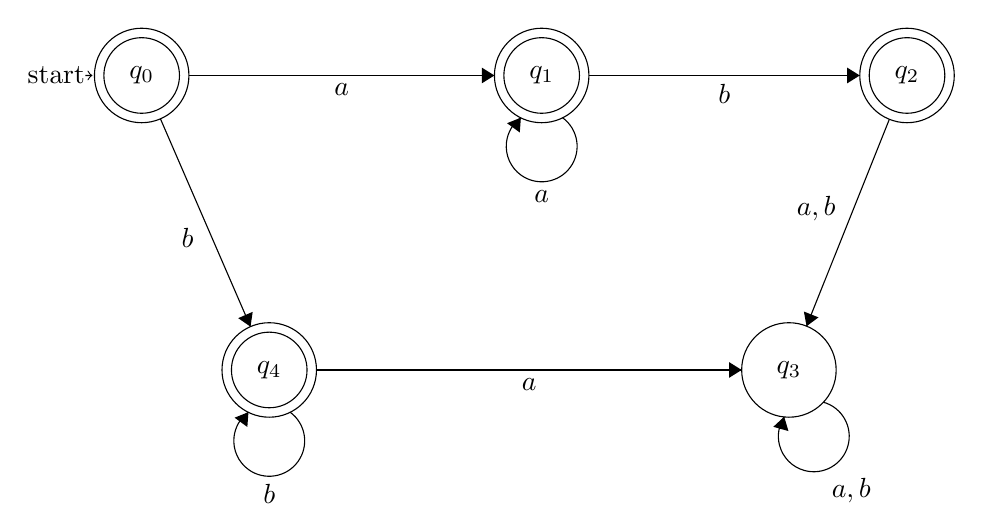
\begin{tikzpicture}[scale=0.2]
\tikzstyle{every node}+=[inner sep=0pt]
\draw [black] (14.3,-12.7) circle (3);
\draw (14.3,-12.7) node {$q_0$};
\draw [black] (14.3,-12.7) circle (2.4);
\draw [black] (39.7,-12.7) circle (3);
\draw (39.7,-12.7) node {$q_1$};
\draw [black] (39.7,-12.7) circle (2.4);
\draw [black] (22.4,-31.4) circle (3);
\draw (22.4,-31.4) node {$q_4$};
\draw [black] (22.4,-31.4) circle (2.4);
\draw [black] (62.9,-12.7) circle (3);
\draw (62.9,-12.7) node {$q_2$};
\draw [black] (62.9,-12.7) circle (2.4);
\draw [black] (55.4,-31.4) circle (3);
\draw (55.4,-31.4) node {$q_3$};
\draw [black] (17.3,-12.7) -- (36.7,-12.7);
\fill [black] (36.7,-12.7) -- (35.9,-12.2) -- (35.9,-13.2);
\draw (27,-13.2) node [below] {$a$};
\draw (11.3,-12.7) node [initial] {$ $};
\draw [black] (41.023,-15.38) arc (54:-234:2.25);
\draw (39.7,-19.95) node [below] {$a$};
\fill [black] (38.38,-15.38) -- (37.5,-15.73) -- (38.31,-16.32);
\draw [black] (42.7,-12.7) -- (59.9,-12.7);
\fill [black] (59.9,-12.7) -- (59.1,-12.2) -- (59.1,-13.2);
\draw (51.3,-13.2) node [below] {$b$};
\draw [black] (61.78,-15.48) -- (56.52,-28.62);
\fill [black] (56.52,-28.62) -- (57.28,-28.06) -- (56.35,-27.69);
\draw (58.4,-21.16) node [left] {$a,b$};
\draw [black] (57.579,-33.445) arc (74.55605:-213.44395:2.25);
\draw (59.36,-38.26) node [below] {$a,b$};
\fill [black] (55.1,-34.37) -- (54.41,-35.01) -- (55.37,-35.28);
\draw [black] (25.4,-31.4) -- (52.4,-31.4);
\fill [black] (52.4,-31.4) -- (51.6,-30.9) -- (51.6,-31.9);
\draw (38.9,-31.9) node [below] {$a$};
\draw [black] (23.723,-34.08) arc (54:-234:2.25);
\draw (22.4,-38.65) node [below] {$b$};
\fill [black] (21.08,-34.08) -- (20.2,-34.43) -- (21.01,-35.02);
\draw [black] (15.49,-15.45) -- (21.21,-28.65);
\fill [black] (21.21,-28.65) -- (21.35,-27.71) -- (20.43,-28.11);
\draw (17.62,-23.02) node [left] {$b$};
\end{tikzpicture}
\end{center}

\subsection*{b.}
\begin{center}
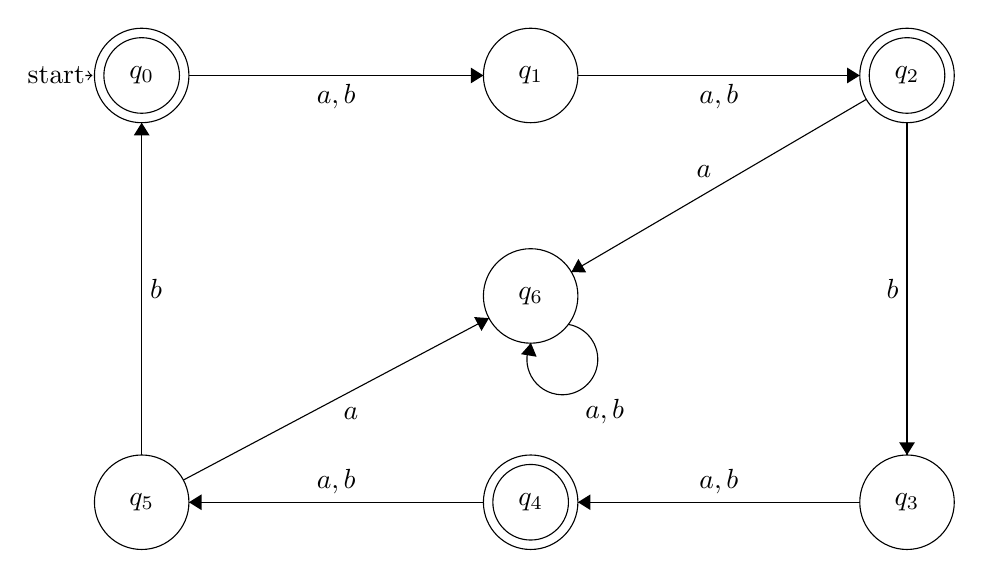
\begin{tikzpicture}[scale=0.2]
\tikzstyle{every node}+=[inner sep=0pt]
\draw [black] (14.3,-12.7) circle (3);
\draw (14.3,-12.7) node {$q_0$};
\draw [black] (14.3,-12.7) circle (2.4);
\draw [black] (39,-12.7) circle (3);
\draw (39,-12.7) node {$q_1$};
\draw [black] (39,-39.8) circle (3);
\draw (39,-39.8) node {$q_4$};
\draw [black] (39,-39.8) circle (2.4);
\draw [black] (62.9,-12.7) circle (3);
\draw (62.9,-12.7) node {$q_2$};
\draw [black] (62.9,-12.7) circle (2.4);
\draw [black] (62.9,-39.8) circle (3);
\draw (62.9,-39.8) node {$q_3$};
\draw [black] (39,-26.7) circle (3);
\draw (39,-26.7) node {$q_6$};
\draw [black] (14.3,-39.8) circle (3);
\draw (14.3,-39.8) node {$q_5$};
\draw [black] (17.3,-12.7) -- (36,-12.7);
\fill [black] (36,-12.7) -- (35.2,-12.2) -- (35.2,-13.2);
\draw (26.65,-13.2) node [below] {$a,b$};
\draw (11.3,-12.7) node [initial] {$ $};
\draw [black] (42,-12.7) -- (59.9,-12.7);
\fill [black] (59.9,-12.7) -- (59.1,-12.2) -- (59.1,-13.2);
\draw (50.95,-13.2) node [below] {$a,b$};
\draw [black] (62.9,-15.7) -- (62.9,-36.8);
\fill [black] (62.9,-36.8) -- (63.4,-36) -- (62.4,-36);
\draw (62.4,-26.25) node [left] {$b$};
\draw [black] (60.31,-14.22) -- (41.59,-25.18);
\fill [black] (41.59,-25.18) -- (42.53,-25.21) -- (42.03,-24.35);
\draw (50.01,-19.2) node [above] {$a$};
\draw [black] (59.9,-39.8) -- (42,-39.8);
\fill [black] (42,-39.8) -- (42.8,-40.3) -- (42.8,-39.3);
\draw (50.95,-39.3) node [above] {$a,b$};
\draw [black] (36,-39.8) -- (17.3,-39.8);
\fill [black] (17.3,-39.8) -- (18.1,-40.3) -- (18.1,-39.3);
\draw (26.65,-39.3) node [above] {$a,b$};
\draw [black] (14.3,-36.8) -- (14.3,-15.7);
\fill [black] (14.3,-15.7) -- (13.8,-16.5) -- (14.8,-16.5);
\draw (14.8,-26.25) node [right] {$b$};
\draw [black] (16.95,-38.39) -- (36.35,-28.11);
\fill [black] (36.35,-28.11) -- (35.41,-28.04) -- (35.88,-28.92);
\draw (27.59,-33.75) node [below] {$a$};
\draw [black] (41.381,-28.505) arc (80.56505:-207.43495:2.25);
\draw (43.7,-33.25) node [below] {$a,b$};
\fill [black] (39.02,-29.69) -- (38.39,-30.4) -- (39.38,-30.56);
\end{tikzpicture}
\end{center}


\subsection*{c.}
\begin{center}
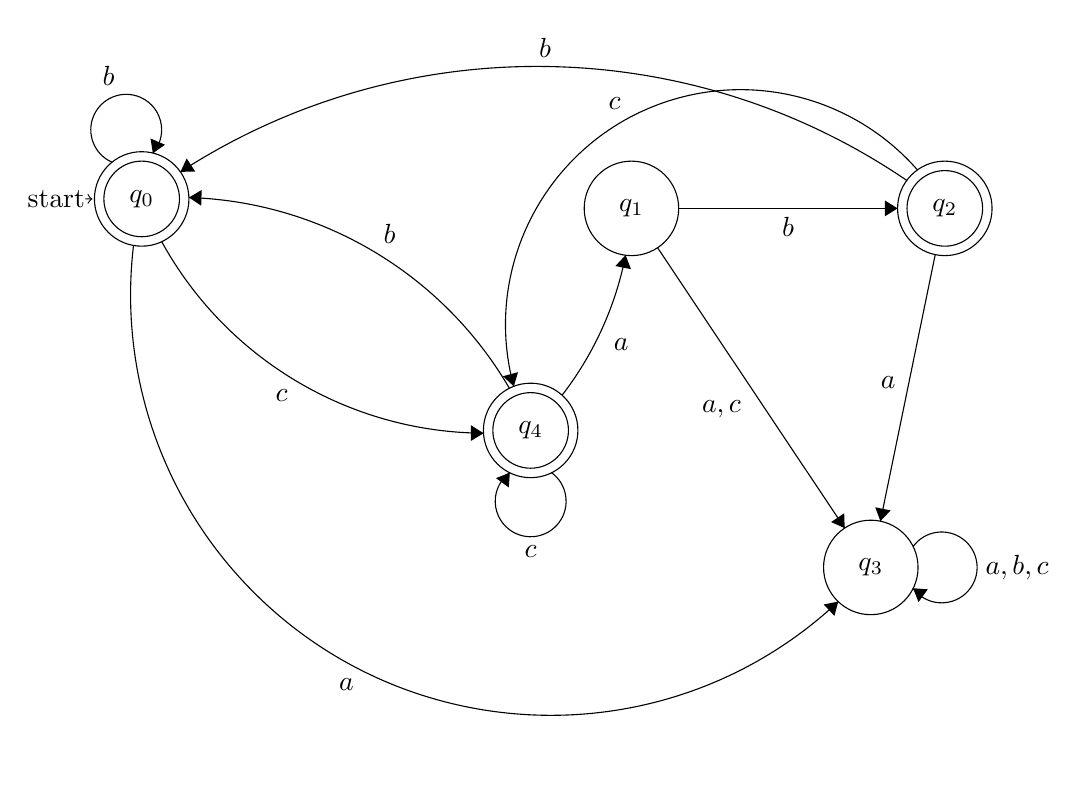
\begin{tikzpicture}[scale=0.2]
\tikzstyle{every node}+=[inner sep=0pt]
\draw [black] (14.3,-12.7) circle (3);
\draw (14.3,-12.7) node {$q_0$};
\draw [black] (14.3,-12.7) circle (2.4);
\draw [black] (45.4,-13.3) circle (3);
\draw (45.4,-13.3) node {$q_1$};
\draw [black] (39,-27.4) circle (3);
\draw (39,-27.4) node {$q_4$};
\draw [black] (39,-27.4) circle (2.4);
\draw [black] (65.3,-13.3) circle (3);
\draw (65.3,-13.3) node {$q_2$};
\draw [black] (65.3,-13.3) circle (2.4);
\draw [black] (60.6,-36.1) circle (3);
\draw (60.6,-36.1) node {$q_3$};
\draw [black] (12.425,-10.373) arc (246.60291:-41.39709:2.25);
\draw (12.19,-5.53) node [above] {$b$};
\draw (11.3,-12.7) node [initial] {$ $};
\fill [black] (15.01,-9.8) -- (15.78,-9.26) -- (14.86,-8.86);
\draw [black] (36.007,-27.575) arc (-90.3094:-151.20788:23.461);
\fill [black] (36.01,-27.58) -- (35.21,-27.07) -- (35.2,-28.07);
\draw (23.19,-24.78) node [below] {$c$};
\draw [black] (17.297,-12.61) arc (88.21326:30.26946:24.449);
\fill [black] (17.3,-12.61) -- (18.08,-13.13) -- (18.11,-12.13);
\draw (30.04,-15.54) node [above] {$b$};
\draw [black] (40.323,-30.08) arc (54:-234:2.25);
\draw (39,-34.65) node [below] {$c$};
\fill [black] (37.68,-30.08) -- (36.8,-30.43) -- (37.61,-31.02);
\draw [black] (45.03,-16.275) arc (-11.13765:-37.68902:21.254);
\fill [black] (45.03,-16.27) -- (44.38,-16.96) -- (45.37,-17.16);
\draw (44.25,-21.97) node [right] {$a$};
\draw [black] (48.4,-13.3) -- (62.3,-13.3);
\fill [black] (62.3,-13.3) -- (61.5,-12.8) -- (61.5,-13.8);
\draw (55.35,-13.8) node [below] {$b$};
\draw [black] (47.06,-15.8) -- (58.94,-33.6);
\fill [black] (58.94,-33.6) -- (58.91,-32.66) -- (58.08,-33.22);
\draw (52.39,-26.03) node [left] {$a,c$};
\draw [black] (64.69,-16.24) -- (61.21,-33.16);
\fill [black] (61.21,-33.16) -- (61.86,-32.48) -- (60.88,-32.28);
\draw (62.21,-24.37) node [left] {$a$};
\draw [black] (63.28,-34.777) arc (144:-144:2.25);
\draw (67.85,-36.1) node [right] {$a,b,c$};
\fill [black] (63.28,-37.42) -- (63.63,-38.3) -- (64.22,-37.49);
\draw [black] (58.532,-38.271) arc (-46.83936:-186.78467:26.685);
\fill [black] (58.53,-38.27) -- (57.61,-38.45) -- (58.29,-39.18);
\draw (27.3,-43.13) node [below] {$a$};
\draw [black] (37.928,-24.604) arc (-164.77776:-318.8288:14.925);
\fill [black] (37.93,-24.6) -- (38.2,-23.7) -- (37.24,-23.96);
\draw (44.34,-7.03) node [above] {$c$};
\draw [black] (16.757,-10.98) arc (122.93202:55.71991:41.673);
\fill [black] (16.76,-10.98) -- (17.7,-10.96) -- (17.16,-10.13);
\draw (39.91,-3.77) node [above] {$b$};
\end{tikzpicture}
\end{center}


\section*{Answer 3}

\subsection*{a.}
We have an NFA N such that:

\begin{center}
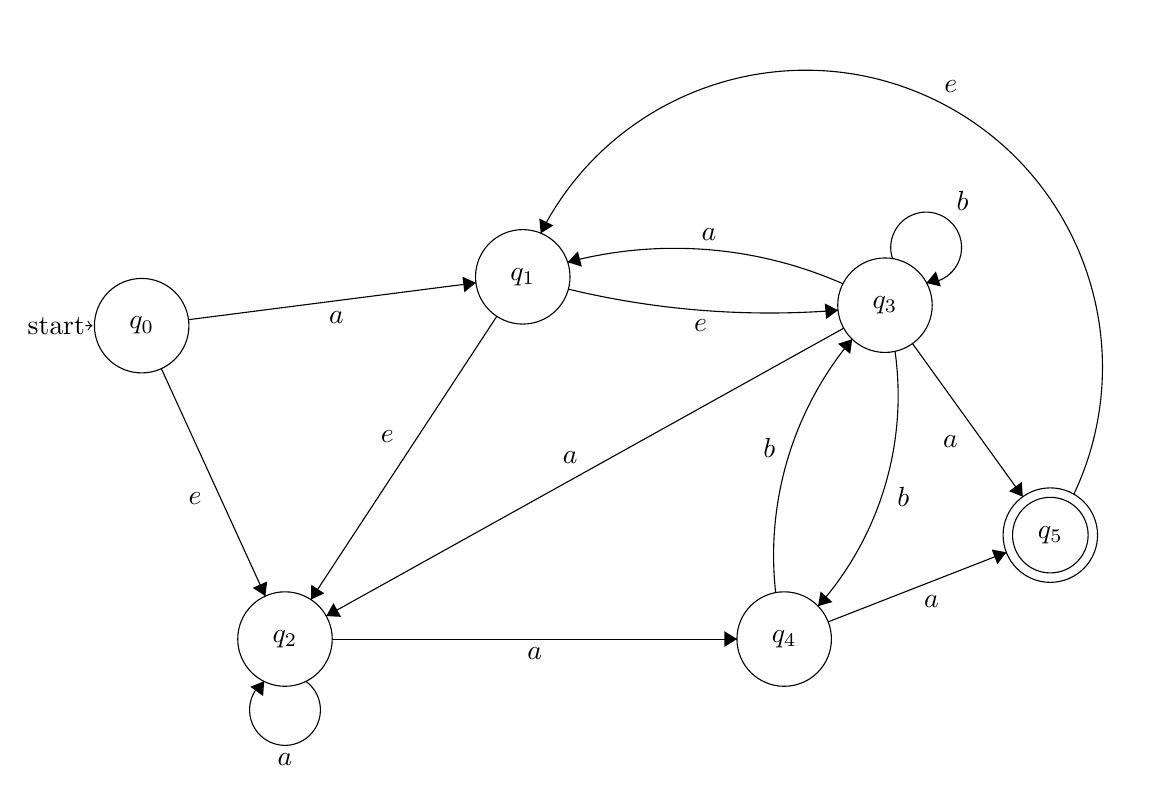
\begin{tikzpicture}[scale=0.2]
\tikzstyle{every node}+=[inner sep=0pt]
\draw [black] (9.5,-19) circle (3);
\draw (9.5,-19) node {$q_0$};
\draw [black] (33.7,-15.9) circle (3);
\draw (33.7,-15.9) node {$q_1$};
\draw [black] (50.3,-38.9) circle (3);
\draw (50.3,-38.9) node {$q_4$};
\draw [black] (56.7,-17.7) circle (3);
\draw (56.7,-17.7) node {$q_3$};
\draw [black] (67.2,-32.3) circle (3);
\draw (67.2,-32.3) node {$q_5$};
\draw [black] (67.2,-32.3) circle (2.4);
\draw [black] (18.6,-38.9) circle (3);
\draw (18.6,-38.9) node {$q_2$};
\draw (6.5,-19) node [initial] {$ $};
\draw [black] (12.48,-18.62) -- (30.72,-16.28);
\fill [black] (30.72,-16.28) -- (29.87,-15.89) -- (29.99,-16.88);
\draw (21.87,-18.04) node [below] {$a$};
\draw [black] (10.75,-21.73) -- (17.35,-36.17);
\fill [black] (17.35,-36.17) -- (17.47,-35.24) -- (16.56,-35.65);
\draw (13.33,-29.97) node [left] {$e$};
\draw [black] (32.05,-18.41) -- (20.25,-36.39);
\fill [black] (20.25,-36.39) -- (21.1,-36) -- (20.27,-35.45);
\draw (25.54,-26.07) node [left] {$e$};
\draw [black] (19.923,-41.58) arc (54:-234:2.25);
\draw (18.6,-46.15) node [below] {$a$};
\fill [black] (17.28,-41.58) -- (16.4,-41.93) -- (17.21,-42.52);
\draw [black] (21.6,-38.9) -- (47.3,-38.9);
\fill [black] (47.3,-38.9) -- (46.5,-38.4) -- (46.5,-39.4);
\draw (34.45,-39.4) node [below] {$a$};
\draw [black] (53.718,-18.022) arc (-85.42099:-103.52881:54.568);
\fill [black] (53.72,-18.02) -- (52.88,-17.59) -- (52.96,-18.58);
\draw (44.99,-18.59) node [below] {$e$};
\draw [black] (36.55,-14.97) arc (104.83315:66.21706:26.512);
\fill [black] (36.55,-14.97) -- (37.45,-15.25) -- (37.2,-14.28);
\draw (45.52,-13.6) node [above] {$a$};
\draw [black] (57.181,-14.751) arc (198.46232:-89.53768:2.25);
\draw (61.63,-11.71) node [above] {$b$};
\fill [black] (59.33,-16.29) -- (60.25,-16.51) -- (59.93,-15.56);
\draw [black] (49.759,-35.952) arc (-173.6169:-219.97984:21.356);
\fill [black] (54.62,-19.86) -- (53.72,-20.15) -- (54.49,-20.79);
\draw (49.77,-26.79) node [left] {$b$};
\draw [black] (57.339,-20.628) arc (8.03814:-41.63488:20.127);
\fill [black] (52.45,-36.81) -- (53.36,-36.55) -- (52.61,-35.88);
\draw (57.45,-29.87) node [right] {$b$};
\draw [black] (53.09,-37.81) -- (64.41,-33.39);
\fill [black] (64.41,-33.39) -- (63.48,-33.22) -- (63.84,-34.15);
\draw (59.65,-36.12) node [below] {$a$};
\draw [black] (58.45,-20.14) -- (65.45,-29.86);
\fill [black] (65.45,-29.86) -- (65.39,-28.92) -- (64.58,-29.51);
\draw (61.36,-26.38) node [left] {$a$};
\draw [black] (34.835,-13.127) arc (153.17951:-25.34784:18.851);
\fill [black] (34.84,-13.13) -- (35.64,-12.64) -- (34.75,-12.19);
\draw (60.88,-4.2) node [above] {$e$};
\draw [black] (54.08,-19.16) -- (21.22,-37.44);
\fill [black] (21.22,-37.44) -- (22.16,-37.49) -- (21.68,-36.62);
\draw (36.71,-27.8) node [above] {$a$};
\end{tikzpicture}
\end{center}

To check if $w_1=abbb$ is in $L(N)$ or not we need this NFA to read $w_1$, namely machine should be on its final state $(q_5)$ when the string is read and no letter to be read is left. Any path which leads to leaf which has an accepting state, means the string is in the language of that NFA. Machine must backtrack to its nondeterministic choice when it fails on any of its choices to read the string. We can demonstrate this computation of the machine with a computational tree:

\begin{center}
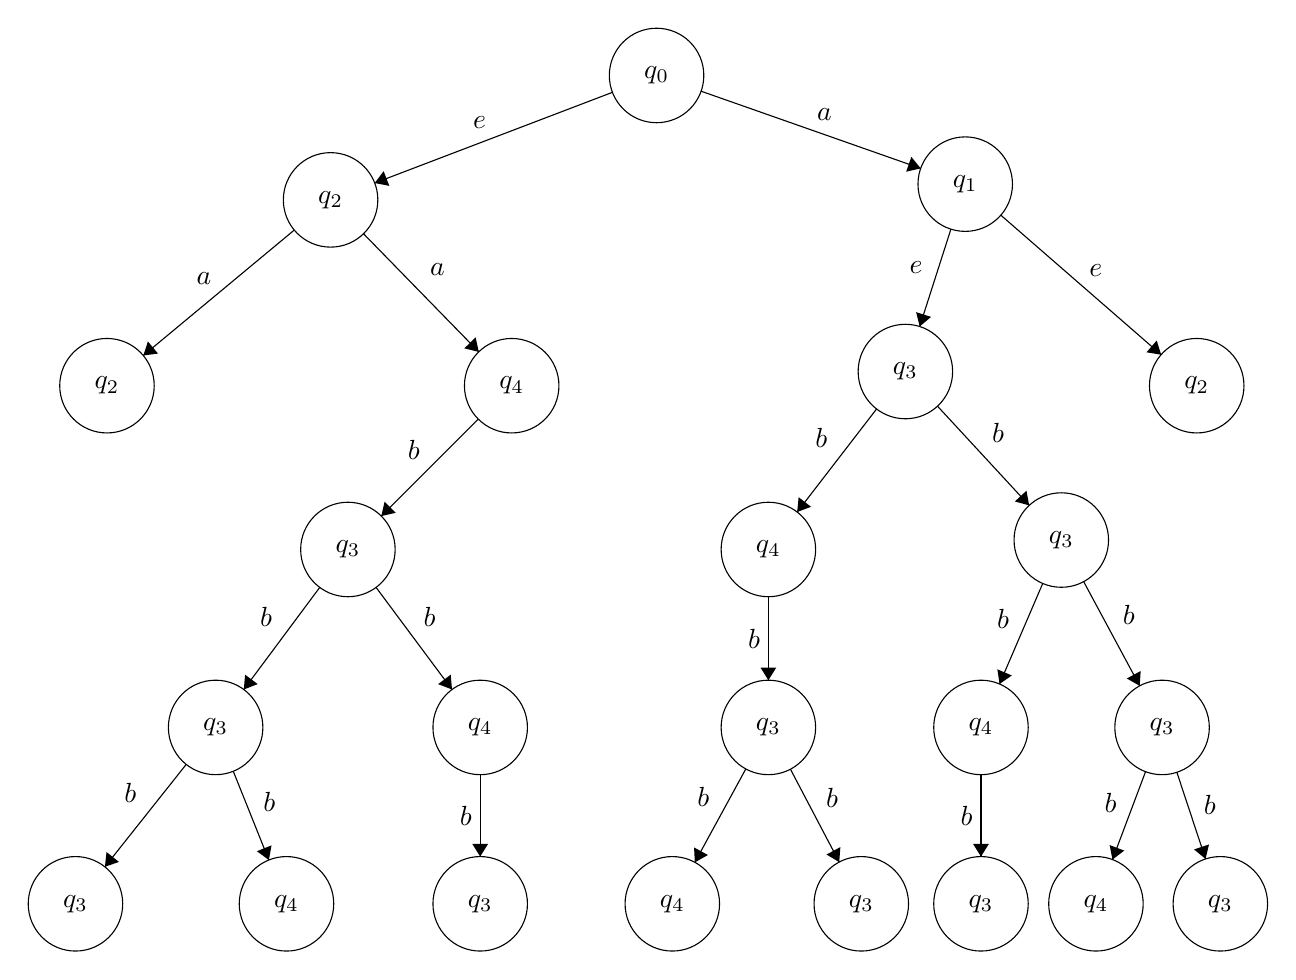
\begin{tikzpicture}[scale=0.2]
\tikzstyle{every node}+=[inner sep=0pt]
\draw [black] (41,-3) circle (3);
\draw (41,-3) node {$q_0$};
\draw [black] (60.6,-9.9) circle (3);
\draw (60.6,-9.9) node {$q_1$};
\draw [black] (31.8,-22.7) circle (3);
\draw (31.8,-22.7) node {$q_4$};
\draw [black] (21.4,-33.1) circle (3);
\draw (21.4,-33.1) node {$q_3$};
\draw [black] (20.3,-10.9) circle (3);
\draw (20.3,-10.9) node {$q_2$};
\draw [black] (6.1,-22.7) circle (3);
\draw (6.1,-22.7) node {$q_2$};
\draw [black] (13,-44.4) circle (3);
\draw (13,-44.4) node {$q_3$};
\draw [black] (4.1,-55.6) circle (3);
\draw (4.1,-55.6) node {$q_3$};
\draw [black] (17.5,-55.6) circle (3);
\draw (17.5,-55.6) node {$q_4$};
\draw [black] (29.8,-44.4) circle (3);
\draw (29.8,-44.4) node {$q_4$};
\draw [black] (29.8,-55.6) circle (3);
\draw (29.8,-55.6) node {$q_3$};
\draw [black] (75.3,-22.7) circle (3);
\draw (75.3,-22.7) node {$q_2$};
\draw [black] (56.8,-21.8) circle (3);
\draw (56.8,-21.8) node {$q_3$};
\draw [black] (48.1,-33.1) circle (3);
\draw (48.1,-33.1) node {$q_4$};
\draw [black] (66.7,-32.5) circle (3);
\draw (66.7,-32.5) node {$q_3$};
\draw [black] (48.1,-44.4) circle (3);
\draw (48.1,-44.4) node {$q_3$};
\draw [black] (42,-55.6) circle (3);
\draw (42,-55.6) node {$q_4$};
\draw [black] (54,-55.6) circle (3);
\draw (54,-55.6) node {$q_3$};
\draw [black] (61.6,-44.4) circle (3);
\draw (61.6,-44.4) node {$q_4$};
\draw [black] (73.1,-44.4) circle (3);
\draw (73.1,-44.4) node {$q_3$};
\draw [black] (61.6,-55.6) circle (3);
\draw (61.6,-55.6) node {$q_3$};
\draw [black] (68.9,-55.6) circle (3);
\draw (68.9,-55.6) node {$q_4$};
\draw [black] (76.8,-55.6) circle (3);
\draw (76.8,-55.6) node {$q_3$};
\draw [black] (38.2,-4.07) -- (23.1,-9.83);
\fill [black] (23.1,-9.83) -- (24.03,-10.01) -- (23.67,-9.08);
\draw (29.76,-6.43) node [above] {$e$};
\draw [black] (17.99,-12.82) -- (8.41,-20.78);
\fill [black] (8.41,-20.78) -- (9.34,-20.66) -- (8.7,-19.89);
\draw (12.25,-16.31) node [above] {$a$};
\draw [black] (43.83,-4) -- (57.77,-8.9);
\fill [black] (57.77,-8.9) -- (57.18,-8.17) -- (56.85,-9.11);
\draw (51.66,-5.92) node [above] {$a$};
\draw [black] (22.39,-13.05) -- (29.71,-20.55);
\fill [black] (29.71,-20.55) -- (29.51,-19.63) -- (28.79,-20.33);
\draw (26.58,-15.33) node [right] {$a$};
\draw [black] (29.68,-24.82) -- (23.52,-30.98);
\fill [black] (23.52,-30.98) -- (24.44,-30.77) -- (23.73,-30.06);
\draw (25.58,-27.42) node [above] {$b$};
\draw [black] (19.61,-35.51) -- (14.79,-41.99);
\fill [black] (14.79,-41.99) -- (15.67,-41.65) -- (14.87,-41.05);
\draw (16.62,-37.36) node [left] {$b$};
\draw [black] (11.13,-46.75) -- (5.97,-53.25);
\fill [black] (5.97,-53.25) -- (6.86,-52.94) -- (6.07,-52.31);
\draw (7.99,-48.58) node [left] {$b$};
\draw [black] (14.12,-47.18) -- (16.38,-52.82);
\fill [black] (16.38,-52.82) -- (16.55,-51.89) -- (15.62,-52.26);
\draw (16,-49.11) node [right] {$b$};
\draw [black] (23.19,-35.51) -- (28.01,-41.99);
\fill [black] (28.01,-41.99) -- (27.93,-41.05) -- (27.13,-41.65);
\draw (26.18,-37.36) node [right] {$b$};
\draw [black] (29.8,-47.4) -- (29.8,-52.6);
\fill [black] (29.8,-52.6) -- (30.3,-51.8) -- (29.3,-51.8);
\draw (29.3,-50) node [left] {$b$};
\draw [black] (62.86,-11.87) -- (73.04,-20.73);
\fill [black] (73.04,-20.73) -- (72.76,-19.83) -- (72.11,-20.58);
\draw (68.9,-15.81) node [above] {$e$};
\draw [black] (59.69,-12.76) -- (57.71,-18.94);
\fill [black] (57.71,-18.94) -- (58.43,-18.33) -- (57.48,-18.03);
\draw (57.93,-15.19) node [left] {$e$};
\draw [black] (54.97,-24.18) -- (49.93,-30.72);
\fill [black] (49.93,-30.72) -- (50.81,-30.39) -- (50.02,-29.78);
\draw (51.88,-26.04) node [left] {$b$};
\draw [black] (58.84,-24) -- (64.66,-30.3);
\fill [black] (64.66,-30.3) -- (64.49,-29.37) -- (63.75,-30.05);
\draw (62.28,-25.69) node [right] {$b$};
\draw [black] (48.1,-36.1) -- (48.1,-41.4);
\fill [black] (48.1,-41.4) -- (48.6,-40.6) -- (47.6,-40.6);
\draw (47.6,-38.75) node [left] {$b$};
\draw [black] (46.67,-47.03) -- (43.43,-52.97);
\fill [black] (43.43,-52.97) -- (44.26,-52.5) -- (43.38,-52.02);
\draw (44.38,-48.82) node [left] {$b$};
\draw [black] (49.5,-47.05) -- (52.6,-52.95);
\fill [black] (52.6,-52.95) -- (52.67,-52) -- (51.79,-52.47);
\draw (51.73,-48.85) node [right] {$b$};
\draw [black] (65.52,-35.26) -- (62.78,-41.64);
\fill [black] (62.78,-41.64) -- (63.56,-41.1) -- (62.64,-40.71);
\draw (63.42,-37.5) node [left] {$b$};
\draw [black] (61.6,-47.4) -- (61.6,-52.6);
\fill [black] (61.6,-52.6) -- (62.1,-51.8) -- (61.1,-51.8);
\draw (61.1,-50) node [left] {$b$};
\draw [black] (68.12,-35.14) -- (71.68,-41.76);
\fill [black] (71.68,-41.76) -- (71.74,-40.82) -- (70.86,-41.29);
\draw (70.58,-37.28) node [right] {$b$};
\draw [black] (72.05,-47.21) -- (69.95,-52.79);
\fill [black] (69.95,-52.79) -- (70.7,-52.22) -- (69.77,-51.87);
\draw (70.24,-49.18) node [left] {$b$};
\draw [black] (74.04,-47.25) -- (75.86,-52.75);
\fill [black] (75.86,-52.75) -- (76.08,-51.83) -- (75.13,-52.15);
\draw (75.72,-49.31) node [right] {$b$};
\end{tikzpicture}
\end{center}

As we can see from the computational tree figure above there is not any leaf in which machine has reached its final state $q_5$, hence we can infer that the string $w_1 \notin L(N)$.

\newpage
\subsection*{b.}
Same as part a, we will use the same NFA to decide if $w_2=ababa$ is in $L(N)$ or not. Let us make the computation with the computational tree:

\begin{center}
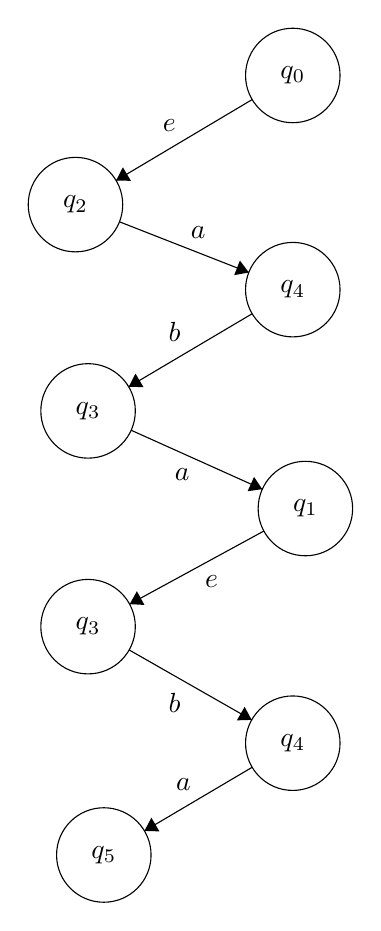
\begin{tikzpicture}[scale=0.2]
\tikzstyle{every node}+=[inner sep=0pt]
\draw [black] (41,-6.3) circle (3);
\draw (41,-6.3) node {$q_0$};
\draw [black] (41,-19.9) circle (3);
\draw (41,-19.9) node {$q_4$};
\draw [black] (28,-27.6) circle (3);
\draw (28,-27.6) node {$q_3$};
\draw [black] (27.2,-14.5) circle (3);
\draw (27.2,-14.5) node {$q_2$};
\draw [black] (41.8,-33.8) circle (3);
\draw (41.8,-33.8) node {$q_1$};
\draw [black] (28,-41.3) circle (3);
\draw (28,-41.3) node {$q_3$};
\draw [black] (41,-48.7) circle (3);
\draw (41,-48.7) node {$q_4$};
\draw [black] (29,-55.8) circle (3);
\draw (29,-55.8) node {$q_5$};
\draw [black] (38.42,-7.83) -- (29.78,-12.97);
\fill [black] (29.78,-12.97) -- (30.72,-12.99) -- (30.21,-12.13);
\draw (33.16,-9.9) node [above] {$e$};
\draw [black] (29.99,-15.59) -- (38.21,-18.81);
\fill [black] (38.21,-18.81) -- (37.64,-18.05) -- (37.28,-18.98);
\draw (35,-16.68) node [above] {$a$};
\draw [black] (38.42,-21.43) -- (30.58,-26.07);
\fill [black] (30.58,-26.07) -- (31.52,-26.09) -- (31.01,-25.23);
\draw (33.5,-23.25) node [above] {$b$};
\draw [black] (30.74,-28.83) -- (39.06,-32.57);
\fill [black] (39.06,-32.57) -- (38.54,-31.79) -- (38.13,-32.7);
\draw (33.98,-31.21) node [below] {$a$};
\draw [black] (39.16,-35.23) -- (30.64,-39.87);
\fill [black] (30.64,-39.87) -- (31.58,-39.92) -- (31.1,-39.05);
\draw (35.84,-38.05) node [below] {$e$};
\draw [black] (30.61,-42.78) -- (38.39,-47.22);
\fill [black] (38.39,-47.22) -- (37.94,-46.39) -- (37.45,-47.25);
\draw (33.5,-45.5) node [below] {$b$};
\draw [black] (38.42,-50.23) -- (31.58,-54.27);
\fill [black] (31.58,-54.27) -- (32.53,-54.3) -- (32.02,-53.43);
\draw (34.06,-51.75) node [above] {$a$};
\end{tikzpicture}
\end{center}

As we can see from the computational tree path figure above there is a configuration of states which leads to final state $q_5$ on the leaf which allows machine to read the string $w_2$, hence we can infer that the string $w_2 \in L(N)$.

\newpage
\section*{Answer 4}

\subsection*{a.}
We have an NFA (N) such that:

\begin{center}
\begin{tikzpicture}[scale=0.2]
\tikzstyle{every node}+=[inner sep=0pt]
\draw [black] (10.8,-14) circle (3);
\draw (10.8,-14) node {$q_0$};
\draw [black] (33.9,-14) circle (3);
\draw (33.9,-14) node {$q_1$};
\draw [black] (48.3,-31.6) circle (3);
\draw (48.3,-31.6) node {$q_3$};
\draw [black] (48.3,-31.6) circle (2.4);
\draw [black] (56.7,-14) circle (3);
\draw (56.7,-14) node {$q_2$};
\draw [black] (56.7,-14) circle (2.4);
\draw [black] (13.8,-14) -- (30.9,-14);
\fill [black] (30.9,-14) -- (30.1,-13.5) -- (30.1,-14.5);
\draw (22.35,-13.5) node [above] {$b$};
\draw [black] (36.629,-12.758) arc (110.92798:69.07202:24.276);
\fill [black] (53.97,-12.76) -- (53.4,-12.01) -- (53.05,-12.94);
\draw (45.3,-10.66) node [above] {$a$};
\draw [black] (53.861,-14.965) arc (-73.99685:-106.00315:31.052);
\fill [black] (36.74,-14.96) -- (37.37,-15.67) -- (37.65,-14.7);
\draw (45.3,-16.67) node [below] {$b$};
\draw (7.8,-14) node [initial] {$ $};
\draw [black] (59.38,-12.677) arc (144:-144:2.25);
\draw (63.95,-14) node [right] {$b$};
\fill [black] (59.38,-15.32) -- (59.73,-16.2) -- (60.32,-15.39);
\draw [black] (55.857,-16.879) arc (-17.97506:-33.05268:51.753);
\fill [black] (50.01,-29.13) -- (50.86,-28.74) -- (50.03,-28.19);
\draw (54.05,-24.26) node [right] {$b$};
\draw [black] (49.623,-34.28) arc (54:-234:2.25);
\draw (48.3,-38.85) node [below] {$a$};
\fill [black] (46.98,-34.28) -- (46.1,-34.63) -- (46.91,-35.22);
\draw [black] (45.31,-31.442) arc (-99.11575:-182.30544:14.091);
\fill [black] (33.46,-16.96) -- (32.93,-17.74) -- (33.93,-17.78);
\draw (36.08,-27.88) node [left] {$b$};
\draw [black] (36.304,-15.793) arc (51.19385:27.38497:41.012);
\fill [black] (47.02,-28.89) -- (47.09,-27.95) -- (46.21,-28.41);
\draw (42.9,-20.35) node [right] {$e$};
\draw [black] (12.901,-11.86) arc (132.72319:47.27681:30.73);
\fill [black] (12.9,-11.86) -- (13.83,-11.68) -- (13.15,-10.95);
\draw (33.75,-3.21) node [above] {$a$};
\end{tikzpicture}
\end{center}

To be able to specify N as a GFA and to apply the state elimination on N, it must have only $1$ final state with no outgoing transitions and its initial state must not have any incoming transitions. Therefore we add $2$ more steps with $e$ transitions to/from the old initial/final states as the new initial and final step respectively. The GFA for N:


\begin{center}
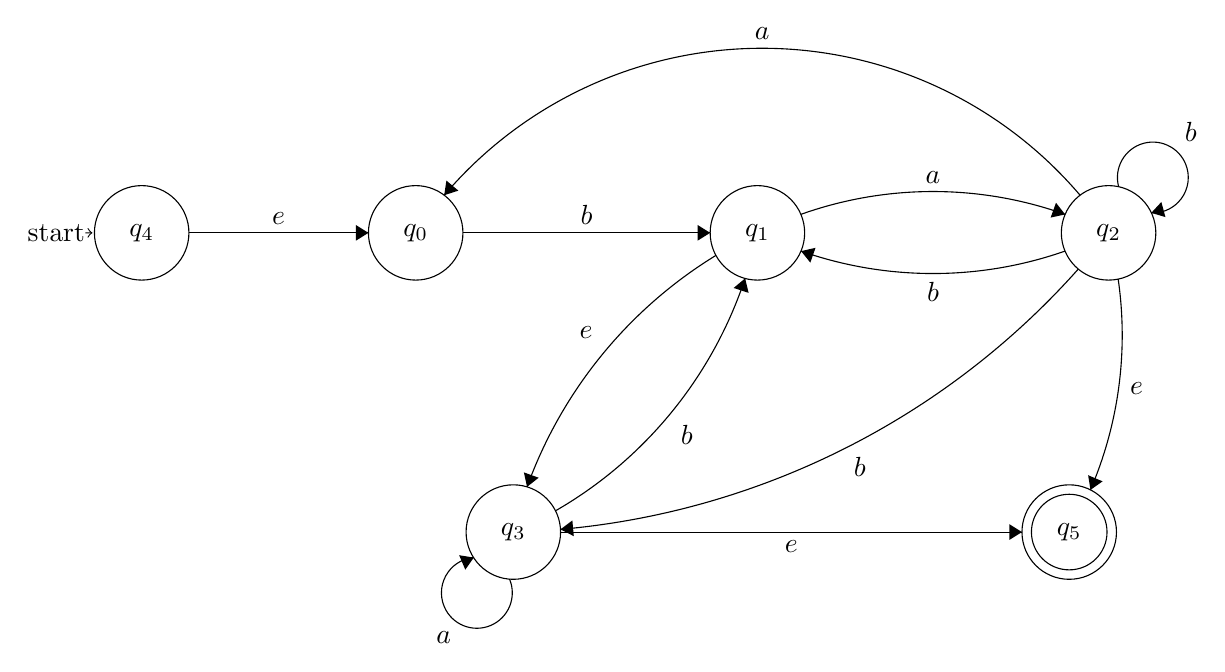
\begin{tikzpicture}[scale=0.2]
\tikzstyle{every node}+=[inner sep=0pt]
\draw [black] (6,-18.4) circle (3);
\draw (6,-18.4) node {$q_4$};
\draw (3,-18.4) node [initial] {$ $};
\draw [black] (23.4,-18.4) circle (3);
\draw (23.4,-18.4) node {$q_0$};
\draw [black] (45.1,-18.4) circle (3);
\draw (45.1,-18.4) node {$q_1$};
\draw [black] (67.4,-18.4) circle (3);
\draw (67.4,-18.4) node {$q_2$};
\draw [black] (64.9,-37.4) circle (3);
\draw (64.9,-37.4) node {$q_5$};
\draw [black] (64.9,-37.4) circle (2.4);
\draw [black] (29.6,-37.4) circle (3);
\draw (29.6,-37.4) node {$q_3$};
\draw [black] (9,-18.4) -- (20.4,-18.4);
\fill [black] (20.4,-18.4) -- (19.6,-17.9) -- (19.6,-18.9);
\draw (14.7,-17.9) node [above] {$e$};
\draw [black] (26.4,-18.4) -- (42.1,-18.4);
\fill [black] (42.1,-18.4) -- (41.3,-17.9) -- (41.3,-18.9);
\draw (34.25,-17.9) node [above] {$b$};
\draw [black] (30.472,-34.531) arc (160.09934:121.48625:28.691);
\fill [black] (30.47,-34.53) -- (31.21,-33.95) -- (30.27,-33.61);
\draw (34.66,-24.73) node [left] {$e$};
\draw [black] (44.317,-21.294) arc (-18.35713:-60.05727:26.754);
\fill [black] (44.32,-21.29) -- (43.59,-21.9) -- (44.54,-22.21);
\draw (40.21,-31.21) node [right] {$b$};
\draw [black] (29.355,-40.378) arc (23.03624:-264.96376:2.25);
\draw (25.18,-43.69) node [below] {$a$};
\fill [black] (27.09,-39.02) -- (26.16,-38.87) -- (26.55,-39.79);
\draw [black] (47.859,-17.226) arc (109.62219:70.37781:24.988);
\fill [black] (64.64,-17.23) -- (64.06,-16.49) -- (63.72,-17.43);
\draw (56.25,-15.27) node [above] {$a$};
\draw [black] (64.634,-19.557) arc (-70.69263:-109.30737:25.357);
\fill [black] (47.87,-19.56) -- (48.46,-20.29) -- (48.79,-19.35);
\draw (56.25,-21.48) node [below] {$b$};
\draw [black] (65.475,-20.7) arc (-41.65667:-84.97097:49.858);
\fill [black] (32.59,-37.23) -- (33.44,-37.66) -- (33.35,-36.66);
\draw (51.61,-32.61) node [below] {$b$};
\draw [black] (32.6,-37.4) -- (61.9,-37.4);
\fill [black] (61.9,-37.4) -- (61.1,-36.9) -- (61.1,-37.9);
\draw (47.25,-37.9) node [below] {$e$};
\draw [black] (68.008,-21.336) arc (8.24549:-23.23721:24.882);
\fill [black] (66.25,-34.72) -- (67.02,-34.18) -- (66.1,-33.79);
\draw (68.73,-28.3) node [right] {$e$};
\draw [black] (68.041,-15.481) arc (195.34019:-92.65981:2.25);
\draw (72.62,-12.63) node [above] {$b$};
\fill [black] (70.11,-17.13) -- (71.01,-17.4) -- (70.75,-16.44);
\draw [black] (25.211,-16.01) arc (139.61239:40.38761:26.507);
\fill [black] (25.21,-16.01) -- (26.11,-15.72) -- (25.35,-15.08);
\draw (45.4,-6.18) node [above] {$a$};
\end{tikzpicture}
\end{center}

\subsection*{b.}
While eliminating states to convert GFA into a regular expression we will consider the following triangular (rule):

\begin{center}
\begin{tikzpicture}[scale=0.2]
\tikzstyle{every node}+=[inner sep=0pt]
\draw [black] (15.5,-14.7) circle (3);
\draw (15.5,-14.7) node {$q_i$};
\draw [black] (36.9,-38.3) circle (3);
\draw (36.9,-38.3) node {$q$};
\draw [black] (58.6,-14.7) circle (3);
\draw (58.6,-14.7) node {$q_j$};
\draw [black] (18.366,-13.815) arc (105.89005:74.10995:68.24);
\fill [black] (55.73,-13.82) -- (55.1,-13.12) -- (54.83,-14.08);
\draw (37.05,-10.71) node [above] {$\delta$};
\draw [black] (33.951,-37.759) arc (-103.92464:-171.67316:24.306);
\fill [black] (33.95,-37.76) -- (33.29,-37.08) -- (33.05,-38.05);
\draw (21.26,-31.95) node [left] {$\alpha$};
\draw [black] (58.68,-17.697) arc (-2.46749:-82.72905:21.532);
\fill [black] (58.68,-17.7) -- (58.15,-18.47) -- (59.14,-18.52);
\draw (53.55,-32.81) node [right] {$\beta$};
\draw [black] (38.223,-40.98) arc (54:-234:2.25);
\draw (36.9,-45.55) node [below] {$\gamma$};
\fill [black] (35.58,-40.98) -- (34.7,-41.33) -- (35.51,-41.92);
\end{tikzpicture}
\end{center}

\newpage
Eliminate q:


\begin{center}
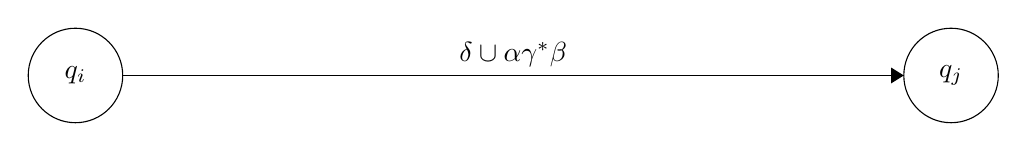
\begin{tikzpicture}[scale=0.2]
\tikzstyle{every node}+=[inner sep=0pt]
\draw [black] (11.1,-21.4) circle (3);
\draw (11.1,-21.4) node {$q_i$};
\draw [black] (66.7,-21.4) circle (3);
\draw (66.7,-21.4) node {$q_j$};
\draw [black] (14.1,-21.4) -- (63.7,-21.4);
\fill [black] (63.7,-21.4) -- (62.9,-20.9) -- (62.9,-21.9);
\draw (38.9,-20.9) node [above] {$\delta\cup\alpha\gamma^*\beta$};
\end{tikzpicture}
\end{center}

So let us start state elimination with eliminating $q_0$:

\begin{center}
\begin{tikzpicture}[scale=0.2]
\tikzstyle{every node}+=[inner sep=0pt]
\draw [black] (7.9,-18.1) circle (3);
\draw (7.9,-18.1) node {$q_4$};
\draw (4.9,-18.1) node [initial] {$ $};
\draw [black] (23.1,-18.1) circle (3);
\draw (23.1,-18.1) node {$q_1$};
\draw [black] (50.9,-18.1) circle (3);
\draw (50.9,-18.1) node {$q_2$};
\draw [black] (68,-18.1) circle (3);
\draw (68,-18.1) node {$q_5$};
\draw [black] (68,-18.1) circle (2.4);
\draw [black] (39.2,-39.3) circle (3);
\draw (39.2,-39.3) node {$q_3$};
\draw [black] (10.9,-18.1) -- (20.1,-18.1);
\fill [black] (20.1,-18.1) -- (19.3,-17.6) -- (19.3,-18.6);
\draw (15.5,-17.6) node [above] {$b$};
\draw [black] (36.659,-37.708) arc (-124.61786:-160.9536:33.692);
\fill [black] (23.95,-20.98) -- (23.74,-21.89) -- (24.69,-21.57);
\draw (28.39,-31.76) node [left] {$b$};
\draw [black] (25.683,-19.624) arc (56.72901:17.69953:31.536);
\fill [black] (38.43,-36.4) -- (38.66,-35.49) -- (37.71,-35.79);
\draw (34.07,-25.52) node [right] {$e$};
\draw [black] (40.523,-41.98) arc (54:-234:2.25);
\draw (39.2,-46.55) node [below] {$a$};
\fill [black] (37.88,-41.98) -- (37,-42.33) -- (37.81,-42.92);
\draw [black] (47.993,-18.839) arc (-77.43255:-102.56745:50.522);
\fill [black] (47.99,-18.84) -- (47.1,-18.53) -- (47.32,-19.5);
\draw (37,-20.55) node [below] {$a$};
\draw [black] (25.907,-17.043) arc (108.20744:71.79256:35.503);
\fill [black] (25.91,-17.04) -- (26.82,-17.27) -- (26.51,-16.32);
\draw (37,-14.77) node [above] {$b\cup ab$};
\draw [black] (50.891,-21.098) arc (-3.992:-53.79545:22.51);
\fill [black] (41.73,-37.69) -- (42.67,-37.63) -- (42.08,-36.82);
\draw (48.81,-31.6) node [right] {$b$};
\draw [black] (51.669,-15.212) arc (192.81407:-95.18593:2.25);
\draw (56.36,-12.53) node [above] {$b$};
\fill [black] (53.66,-16.95) -- (54.55,-17.26) -- (54.33,-16.29);
\draw [black] (53.9,-18.1) -- (65,-18.1);
\fill [black] (65,-18.1) -- (64.2,-17.6) -- (64.2,-18.6);
\draw (59.45,-17.6) node [above] {$e$};
\draw [black] (67.119,-20.966) arc (-20.14734:-87.13826:28.036);
\fill [black] (67.12,-20.97) -- (66.37,-21.55) -- (67.31,-21.89);
\draw (58.37,-34.39) node [below] {$e$};
\end{tikzpicture}
\end{center}

Now eliminate $q_1$:

\begin{center}
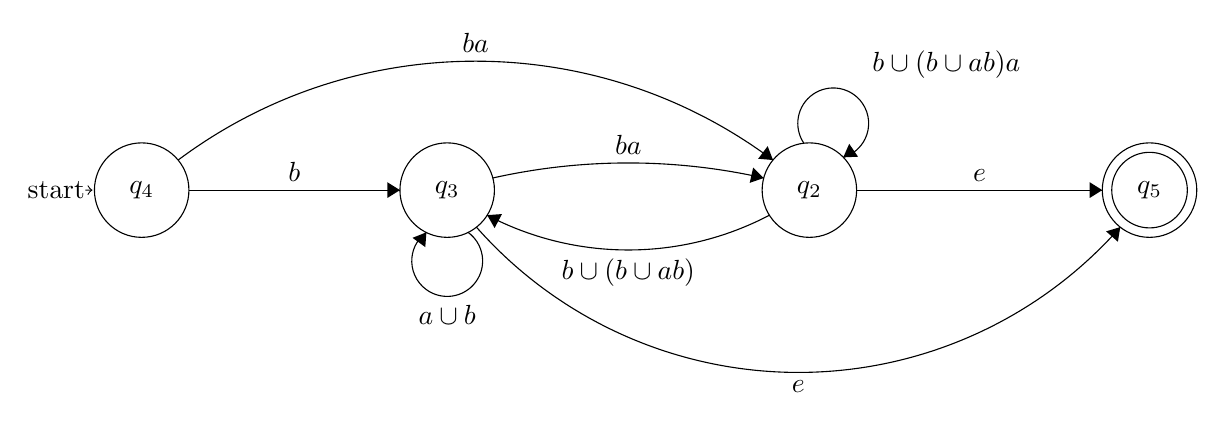
\begin{tikzpicture}[scale=0.2]
\tikzstyle{every node}+=[inner sep=0pt]
\draw [black] (7.9,-18.1) circle (3);
\draw (7.9,-18.1) node {$q_4$};
\draw (4.9,-18.1) node [initial] {$ $};
\draw [black] (27.3,-18.1) circle (3);
\draw (27.3,-18.1) node {$q_3$};
\draw [black] (50.3,-18.1) circle (3);
\draw (50.3,-18.1) node {$q_2$};
\draw [black] (71.9,-18.1) circle (3);
\draw (71.9,-18.1) node {$q_5$};
\draw [black] (71.9,-18.1) circle (2.4);
\draw [black] (10.9,-18.1) -- (24.3,-18.1);
\fill [black] (24.3,-18.1) -- (23.5,-17.6) -- (23.5,-18.6);
\draw (17.6,-17.6) node [above] {$b$};
\draw [black] (53.3,-18.1) -- (68.9,-18.1);
\fill [black] (68.9,-18.1) -- (68.1,-17.6) -- (68.1,-18.6);
\draw (61.1,-17.6) node [above] {$e$};
\draw [black] (28.623,-20.78) arc (54:-234:2.25);
\draw (27.3,-25.35) node [below] {$a\cup b$};
\fill [black] (25.98,-20.78) -- (25.1,-21.13) -- (25.91,-21.72);
\draw [black] (10.214,-16.192) arc (126.78691:53.21309:31.538);
\fill [black] (47.99,-16.19) -- (47.65,-15.31) -- (47.05,-16.11);
\draw (29.1,-9.41) node [above] {$ba$};
\draw [black] (30.199,-17.33) arc (102.67626:77.32374:39.196);
\fill [black] (47.4,-17.33) -- (46.73,-16.67) -- (46.51,-17.64);
\draw (38.8,-15.87) node [above] {$ba$};
\draw [black] (47.762,-19.694) arc (-62.3182:-117.6818:19.292);
\fill [black] (29.84,-19.69) -- (30.31,-20.51) -- (30.78,-19.62);
\draw (38.8,-22.4) node [below] {$b\cup(b\cup ab)$};
\draw [black] (70.042,-20.454) arc (-41.43286:-138.56714:27.266);
\fill [black] (70.04,-20.45) -- (69.14,-20.72) -- (69.89,-21.38);
\draw (49.6,-30.18) node [below] {$e$};
\draw [black] (49.956,-15.132) arc (214.34618:-73.65382:2.25);
\draw (59,-11.04) node [above] {$b\cup(b\cup ab)a$};
\fill [black] (52.45,-16.02) -- (53.39,-15.98) -- (52.83,-15.16);
\end{tikzpicture}
\end{center}

\newpage
Now eliminate $q_3$:

\begin{center}
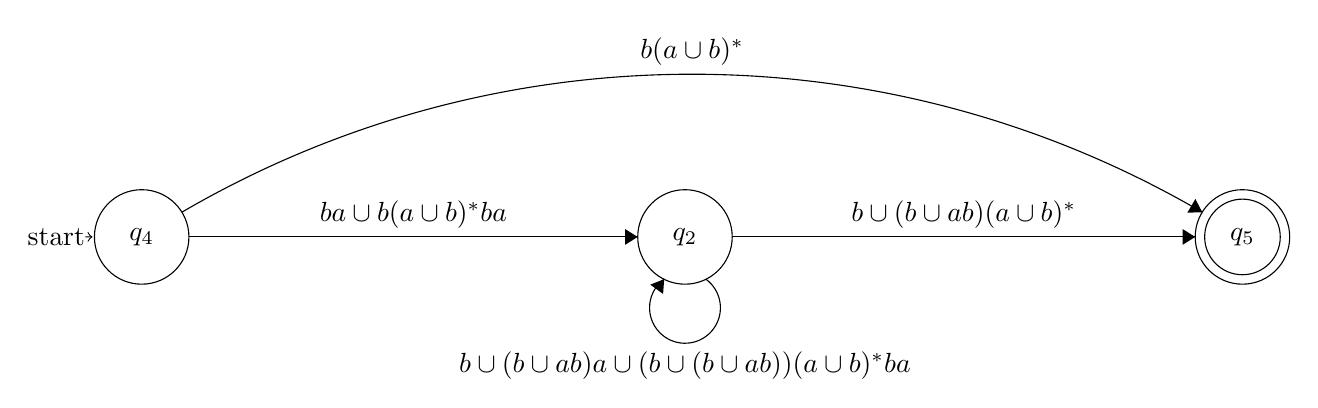
\begin{tikzpicture}[scale=0.2]
\tikzstyle{every node}+=[inner sep=0pt]
\draw [black] (5.1,-18.1) circle (3);
\draw (5.1,-18.1) node {$q_4$};
\draw (2.1,-18.1) node [initial] {$ $};
\draw [black] (39.6,-18.1) circle (3);
\draw (39.6,-18.1) node {$q_2$};
\draw [black] (75,-18.1) circle (3);
\draw (75,-18.1) node {$q_5$};
\draw [black] (75,-18.1) circle (2.4);
\draw [black] (7.655,-16.528) arc (120.27107:59.72893:64.265);
\fill [black] (72.45,-16.53) -- (72.01,-15.69) -- (71.5,-16.56);
\draw (40.05,-7.27) node [above] {$b(a\cup b)^*$};
\draw [black] (8.1,-18.1) -- (36.6,-18.1);
\fill [black] (36.6,-18.1) -- (35.8,-17.6) -- (35.8,-18.6);
\draw (22.35,-17.6) node [above] {$ba\cup b(a\cup b)^*ba$};
\draw [black] (40.923,-20.78) arc (54:-234:2.25);
\draw (39.6,-25.35) node [below] {$b\cup (b\cup ab)a\cup (b\cup (b\cup ab))(a\cup b)^*ba$};
\fill [black] (38.28,-20.78) -- (37.4,-21.13) -- (38.21,-21.72);
\draw [black] (42.6,-18.1) -- (72,-18.1);
\fill [black] (72,-18.1) -- (71.2,-17.6) -- (71.2,-18.6);
\draw (57.3,-17.6) node [above] {$b\cup (b\cup ab)(a\cup b)^*$};
\end{tikzpicture}
\end{center}

Now finally eliminate $q_2$:


\begin{center}
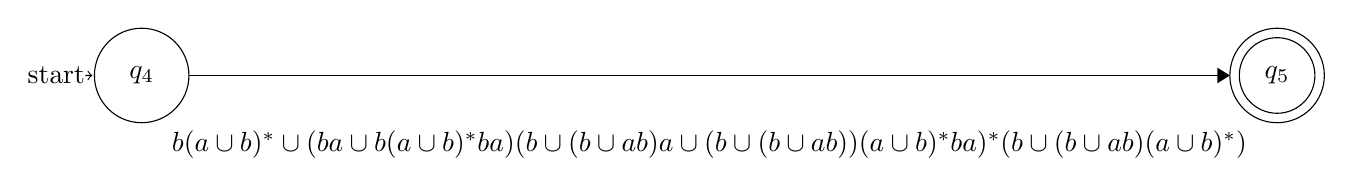
\begin{tikzpicture}[scale=0.2]
\tikzstyle{every node}+=[inner sep=0pt]
\draw [black] (4.2,-18.1) circle (3);
\draw (4.2,-18.1) node {$q_4$};
\draw (1.2,-18.1) node [initial] {$ $};
\draw [black] (76.3,-18.1) circle (3);
\draw (76.3,-18.1) node {$q_5$};
\draw [black] (76.3,-18.1) circle (2.4);
\draw [black] (7.2,-18.1) -- (73.3,-18.1);
\fill [black] (73.3,-18.1) -- (72.5,-17.6) -- (72.5,-18.6);
\draw (40.25,-21.6) node [below] {$b(a\cup b)^*\cup (ba\cup b(a\cup b)^*ba)(b\cup (b\cup ab)a\cup (b\cup (b\cup ab))(a\cup b)^*ba)^*(b\cup (b\cup ab)(a\cup b)^*)$};
\end{tikzpicture}
\end{center}

Therefore the converted form of GFA into regular expression is:\\

$b(a\cup b)^*\cup (ba\cup b(a\cup b)^*ba)(b\cup (b\cup ab)a\cup (b\cup (b\cup ab))(a\cup b)^*ba)^*(b\cup (b\cup ab)(a\cup b)^*)$

\newpage

\section*{Answer 5}

\subsection*{a.}
We have an NFA N such that:

\begin{center}
\begin{tikzpicture}[scale=0.2]
\tikzstyle{every node}+=[inner sep=0pt]
\draw [black] (8.6,-18) circle (3);
\draw (8.6,-18) node {$q_0$};
\draw (5.6,-18) node [initial] {$ $};
\draw [black] (41.2,-18) circle (3);
\draw (41.2,-18) node {$q_1$};
\draw [black] (62.8,-30.4) circle (3);
\draw (62.8,-30.4) node {$q_3$};
\draw [black] (62.8,-30.4) circle (2.4);
\draw [black] (26.7,-36.7) circle (3);
\draw (26.7,-36.7) node {$q_2$};
\draw [black] (11.44,-17.036) arc (106.89531:73.10469:46.313);
\fill [black] (38.36,-17.04) -- (37.74,-16.32) -- (37.45,-17.28);
\draw (24.9,-14.54) node [above] {$a,e$};
\draw [black] (23.731,-37.092) arc (-88.14365:-183.72453:15.16);
\fill [black] (23.73,-37.09) -- (22.91,-36.62) -- (22.95,-37.62);
\draw (11.82,-33.96) node [left] {$b,e$};
\draw [black] (60.322,-32.09) arc (-57.79595:-102.40546:41.08);
\fill [black] (60.32,-32.09) -- (59.38,-32.09) -- (59.91,-32.94);
\draw (45.93,-38.39) node [below] {$a$};
\draw [black] (44.194,-18.165) arc (83.36817:36.9138:24.785);
\fill [black] (44.19,-18.17) -- (44.93,-18.75) -- (45.05,-17.76);
\draw (55.36,-20.79) node [above] {$b,e$};
\end{tikzpicture}
\end{center}

To find an equivalent DFA M such that $L(M) = L(N)$ we will use subset construction algorithm. Firstly, Since $N$ has 5 states, $M$ will have $2^{5}=32$ states. However, only a few of these states will be relevant to the operation of $M$-namely those states that can be reached from state $s'$ by reading some input string. Obviously, any state in $K'$ that is not reachable from $s'$ is irrelevant to the operation of $M$ and to the language accepted by it. We shall build the reachable part of $N$ by starting from $s'$ and introducing a new state only when it is needed as the value of $\delta(q,x)$ for some state $q\in K'$ already introduced and some $x \in \Sigma$.\\
So let's define every $E(q)$ for each state $q$ of $N$:
\begin{align*}
	E(q_0) &= \{q_0,q_1,q_2\} \\
	E(q_1) &= \{q_1\} \\
	E(q_2) &= \{q_2\} \\
	E(q_3) &= \{q_1,q_3\} \\
\end{align*}

Since $s' = E(q_0) = \{q_0,q_1,q_2\}$,
$(q_0,a,q_1), (q_2,a,q_3)$
are all transitions $(q,a,p)$ for some $q\in s'$. It follows that
$$\delta ' (s',a) = E(q_1)\cup E(q_3) = \{ q_1,q_3\}.$$
Similarly,
$$(q_0,b,q_2)$$
is the transition from $(q,b,p)$ for some $q\in s'$, so
$$\delta '(s',b) = E(q_2) = \{q_2\}.$$
After this operations we have:

\begin{center}
\begin{tikzpicture}[scale=0.2]
\tikzstyle{every node}+=[inner sep=0pt]
\draw [black] (10.5,-13.7) circle (3);
\draw (10.5,-13.7) node {$\{q_0,q_1,q_2\}$};
\draw (6.5,-13.7) node [initial] {$ $};
\draw [black] (41.2,-11.9) circle (3);
\draw (41.2,-11.9) node {$\{q_1,q_3\}$};
\draw [black] (41.2,-11.9) circle (2.4);
\draw [black] (20,-34.5) circle (3);
\draw (20,-34.5) node {$\{q_2\}$};
\draw [black] (13.267,-12.543) arc (110.65239:76.05865:42.197);
\fill [black] (38.32,-11.07) -- (37.66,-10.4) -- (37.42,-11.37);
\draw (25.61,-9.35) node [above] {$a$};
\draw [black] (17.39,-33.029) arc (-124.34152:-186.5632:17.439);
\fill [black] (17.39,-33.03) -- (17.01,-32.16) -- (16.45,-32.99);
\draw (10.65,-26.89) node [left] {$b$};
\end{tikzpicture}
\end{center}

Repeating this calculation for the newly introduced states, we have the following;
\begin{align*}
\delta'(\{q_1,q_3\},a) &= \emptyset = \{\} \\
\delta'(\{q_1,q_3\},b) &= E(q_1) = \{ q_1\} \\
\delta'(\{q_2\},a) &= E(q_3) = \{ q_1,q_3\} \\
\delta'(\{q_2\},b) &= \emptyset = \{\} \\
\delta'(\{q_1\},a) &= \emptyset = \{\} \\
\delta'(\{q_1\},b) &= \emptyset = \{\} \\
\end{align*}

The relevant part of M will be our new DFA. $F'$, the set of final states, contains each set of states of which $q_3$ is a member, since $q_3$ is the sole member of $F$; so all states which contains $q_3$ will be the final states. Step by step our new DFA:

\begin{center}
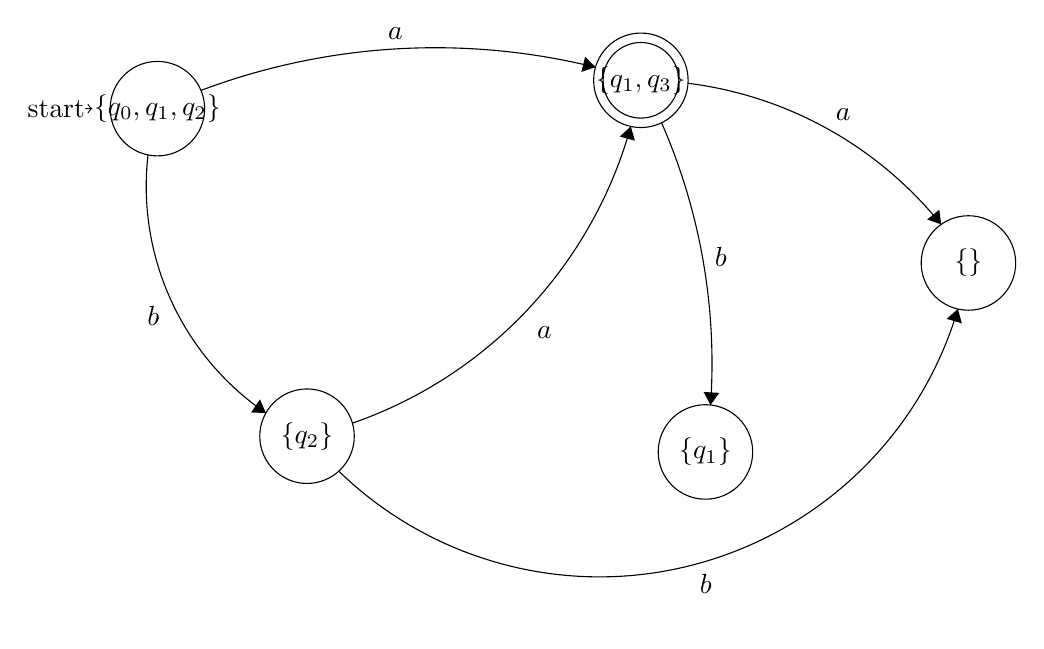
\begin{tikzpicture}[scale=0.2]
\tikzstyle{every node}+=[inner sep=0pt]
\draw [black] (10.5,-13.7) circle (3);
\draw (10.5,-13.7) node {$\{q_0,q_1,q_2\}$};
\draw (6.5,-13.7) node [initial] {$ $};
\draw [black] (41.2,-11.9) circle (3);
\draw (41.2,-11.9) node {$\{q_1,q_3\}$};
\draw [black] (41.2,-11.9) circle (2.4);
\draw [black] (20,-34.5) circle (3);
\draw (20,-34.5) node {$\{q_2\}$};
\draw [black] (45.3,-35.5) circle (3);
\draw (45.3,-35.5) node {$\{q_1\}$};
\draw [black] (62,-23.5) circle (3);
\draw (62,-23.5) node {$\{\}$};
\draw [black] (13.267,-12.543) arc (110.65239:76.05865:42.197);
\fill [black] (38.32,-11.07) -- (37.66,-10.4) -- (37.42,-11.37);
\draw (25.61,-9.35) node [above] {$a$};
\draw [black] (17.39,-33.029) arc (-124.34152:-186.5632:17.439);
\fill [black] (17.39,-33.03) -- (17.01,-32.16) -- (16.45,-32.99);
\draw (10.65,-26.89) node [left] {$b$};
\draw [black] (40.557,-14.829) arc (-15.48293:-70.85558:27.801);
\fill [black] (40.56,-14.83) -- (39.86,-15.47) -- (40.82,-15.73);
\draw (34.57,-27.89) node [right] {$a$};
\draw [black] (42.512,-14.597) arc (23.67429:-3.96316:38.077);
\fill [black] (45.62,-32.52) -- (46.18,-31.75) -- (45.18,-31.69);
\draw (45.87,-23.12) node [right] {$b$};
\draw [black] (44.192,-12.089) arc (82.87863:38.82523:24.538);
\fill [black] (60.27,-21.05) -- (60.15,-20.12) -- (59.38,-20.74);
\draw (54.04,-14.51) node [above] {$a$};
\draw [black] (61.331,-26.423) arc (-16.50284:-134.14438:23.752);
\fill [black] (61.33,-26.42) -- (60.62,-27.05) -- (61.58,-27.33);
\draw (45.33,-43.22) node [below] {$b$};
\end{tikzpicture}
\end{center}

And finally:

\begin{center}
\begin{tikzpicture}[scale=0.2]
\tikzstyle{every node}+=[inner sep=0pt]
\draw [black] (10.9,-14.1) circle (3);
\draw (10.9,-14.1) node {$\{q_0,q_1,q_2\}$};
\draw (6.5,-14.1) node [initial] {$ $};
\draw [black] (41.2,-11.9) circle (3);
\draw (41.2,-11.9) node {$\{q_1,q_3\}$};
\draw [black] (41.2,-11.9) circle (2.4);
\draw [black] (20,-34.5) circle (3);
\draw (20,-34.5) node {$\{q_2\}$};
\draw [black] (46,-33.7) circle (3);
\draw (46,-33.7) node {$\{q_1\}$};
\draw [black] (66.5,-21.7) circle (3);
\draw (66.5,-21.7) node {$\{\}$};
\draw [black] (13.647,-12.895) arc (111.60878:76.69682:41.215);
\fill [black] (38.31,-11.1) -- (37.64,-10.43) -- (37.41,-11.41);
\draw (25.74,-9.54) node [above] {$a$};
\draw [black] (17.386,-33.036) arc (-124.39032:-187.52845:16.746);
\fill [black] (17.39,-33.04) -- (17.01,-32.17) -- (16.44,-33);
\draw (10.83,-27.03) node [left] {$b$};
\draw [black] (40.58,-14.834) arc (-15.06697:-71.27153:27.449);
\fill [black] (40.58,-14.83) -- (39.89,-15.48) -- (40.85,-15.74);
\draw (34.63,-27.94) node [right] {$a$};
\draw [black] (42.402,-14.648) arc (21.89276:2.94213:49.924);
\fill [black] (45.94,-30.7) -- (46.39,-29.88) -- (45.4,-29.93);
\draw (45.58,-22.16) node [right] {$b$};
\draw [black] (44.198,-11.993) arc (85.87098:51.78109:36.629);
\fill [black] (64.22,-19.75) -- (63.9,-18.86) -- (63.28,-19.65);
\draw (55.68,-13.85) node [above] {$a$};
\draw [black] (64.36,-23.802) arc (-47.53164:-71.78186:42.697);
\fill [black] (64.36,-23.8) -- (63.43,-23.97) -- (64.11,-24.71);
\draw (58.79,-29.66) node [below] {$a,b$};
\draw [black] (68.101,-19.177) arc (175.32869:-112.67131:2.25);
\draw (72.9,-16.92) node [right] {$a,b$};
\fill [black] (69.48,-21.44) -- (70.23,-22) -- (70.31,-21);
\draw [black] (66.543,-24.698) arc (-2.66707:-146.55179:24.571);
\fill [black] (66.54,-24.7) -- (66.01,-25.47) -- (67.01,-25.52);
\draw (49.3,-47.8) node [below] {$b$};
\end{tikzpicture}
\end{center}

\subsection*{b.}
The language $\bar{L}$ where $L = L(N)$ (complementation algorithm) requires N to be an equivalent DFA, therefore we will use the equivalent DFA M which we found on part a by subset construction algorithm. First let us demonstrate $\bar{L}$ by swapping all final states and non-final states:

\begin{center}
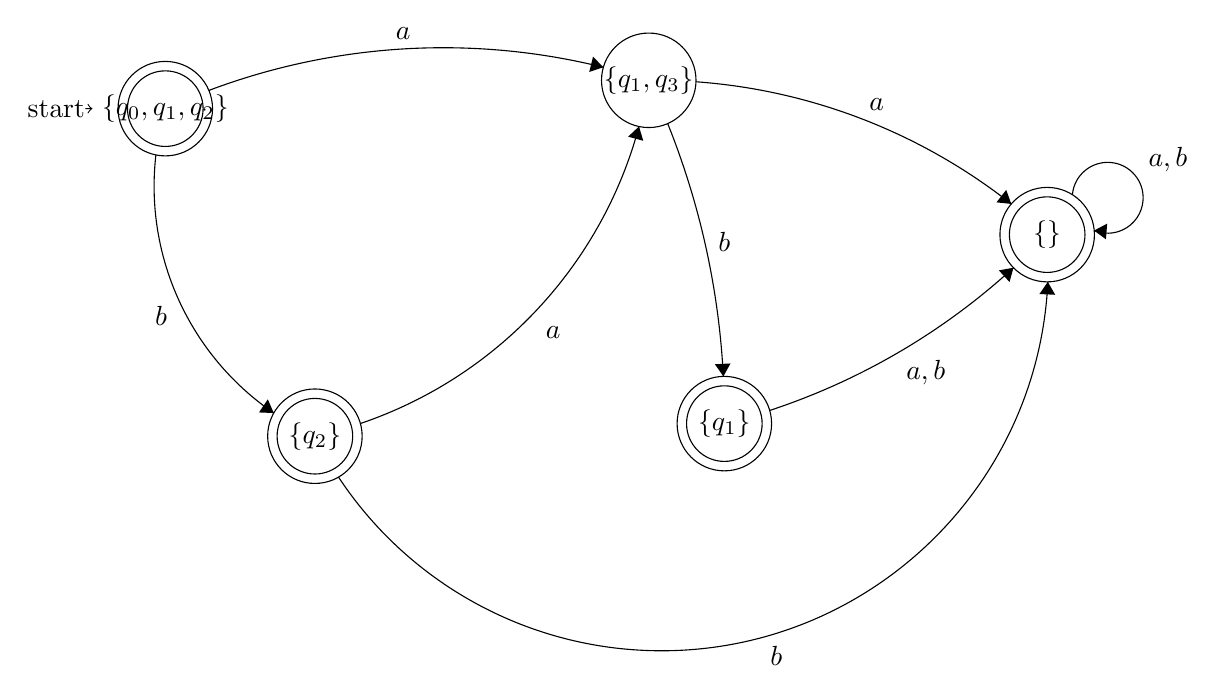
\begin{tikzpicture}[scale=0.2]
\tikzstyle{every node}+=[inner sep=0pt]
\draw [black] (10.5,-13.7) circle (3);
\draw (10.5,-13.7) node {$\{q_0,q_1,q_2\}$};
\draw (6,-13.7) node [initial] {$ $};
\draw [black] (10.5,-13.7) circle (2.4);
\draw [black] (41.2,-11.9) circle (3);
\draw (41.2,-11.9) node {$\{q_1,q_3\}$};
\draw [black] (20,-34.5) circle (3);
\draw (20,-34.5) node {$\{q_2\}$};
\draw [black] (20,-34.5) circle (2.4);
\draw [black] (46,-33.7) circle (3);
\draw (46,-33.7) node {$\{q_1\}$};
\draw [black] (46,-33.7) circle (2.4);
\draw [black] (66.5,-21.7) circle (3);
\draw (66.5,-21.7) node {$\{\}$};
\draw [black] (66.5,-21.7) circle (2.4);
\draw [black] (13.267,-12.543) arc (110.65239:76.05865:42.197);
\fill [black] (38.32,-11.07) -- (37.66,-10.4) -- (37.42,-11.37);
\draw (25.61,-9.35) node [above] {$a$};
\draw [black] (17.39,-33.029) arc (-124.34152:-186.5632:17.439);
\fill [black] (17.39,-33.03) -- (17.01,-32.16) -- (16.45,-32.99);
\draw (10.65,-26.89) node [left] {$b$};
\draw [black] (40.58,-14.834) arc (-15.06697:-71.27153:27.449);
\fill [black] (40.58,-14.83) -- (39.89,-15.48) -- (40.85,-15.74);
\draw (34.63,-27.94) node [right] {$a$};
\draw [black] (42.402,-14.648) arc (21.89276:2.94213:49.924);
\fill [black] (45.94,-30.7) -- (46.39,-29.88) -- (45.4,-29.93);
\draw (45.58,-22.16) node [right] {$b$};
\draw [black] (44.198,-11.993) arc (85.87098:51.78109:36.629);
\fill [black] (64.22,-19.75) -- (63.9,-18.86) -- (63.28,-19.65);
\draw (55.68,-13.85) node [above] {$a$};
\draw [black] (64.36,-23.802) arc (-47.53164:-71.78186:42.697);
\fill [black] (64.36,-23.8) -- (63.43,-23.97) -- (64.11,-24.71);
\draw (58.79,-29.66) node [below] {$a,b$};
\draw [black] (68.101,-19.177) arc (175.32869:-112.67131:2.25);
\draw (72.9,-16.92) node [right] {$a,b$};
\fill [black] (69.48,-21.44) -- (70.23,-22) -- (70.31,-21);
\draw [black] (66.543,-24.698) arc (-2.66707:-146.55179:24.571);
\fill [black] (66.54,-24.7) -- (66.01,-25.47) -- (67.01,-25.52);
\draw (49.3,-47.8) node [below] {$b$};
\end{tikzpicture}
\end{center}

In order to find a regular expression for the language $\bar{L}$ where $L = L(N)$ (we will use the DFA equivalent of N which is M), we need to generate a GFA for the automaton and then step by step convert it to a regular expression as we did in Question 4. By doing this, at the end there will only be two nodes and one transition, where the transition's expression will be our regular expression, which is:
\begin{center}
$(b\cup (ab\cup bab))\cup ((aa\cup b(b\cup aa))\cup (((ab\cup bab)(a\cup b))( a\cup b)^*)$\\
\end{center}

Since we took the complement of language $L$ to construct the language $\bar{L}$, the complementation property of the language is using set notation and we write it as:
\begin{center}
$\bar{L}=\{w\in \{a,b\}^*: w\in U$ $and$ $w\notin L\}$
\end{center}
where $U$ is the set of all languages that can be composed by any number of the symbols over the alphabet $\Sigma = \{a,b\}$

\newpage
\section*{Answer 6}
Let $L_1$ and $L_2$ two arbitrary regular languages and let $M_1=(K_1,\Sigma,\Delta_1,s_1,F_1)$ and $M_2=(K_2,\Sigma,\Delta_2,s_2,F_2)$ NFA's of the languages $L_1$ and $L_2$ respectively. To prove that class of regular languages is closed under set difference operation we will construct an NFA for the language $L_1-L_2$. This language will have an automata that accepts strings when $L_1$ accepts and $L_2$ does not. This operation corresponds to $(\bar{L_1} \cup L_2)'$ and that is equivalent to $L_1 \cap \bar{L_2}$. Since the class of regular languages are closed under complementation, union and intersection, the set difference operation is also closed and reachable from these basic set of operations. We can easily observe that $L_1-L_2 = L_1 \cap\bar{L_2}=(\bar{L_1} \cup L_2)'$ by the Venn Diagram of the language $L_1-L_2$ below:

\begin{center}
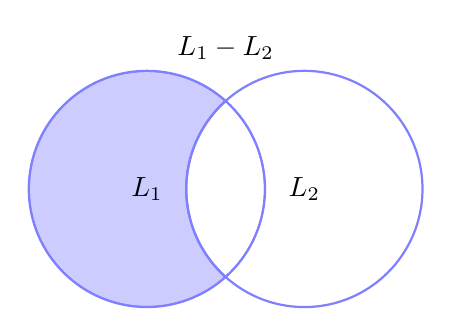
\begin{tikzpicture}
    \begin{scope}
        \clip \firstcircle;
        \draw[filled, even odd rule] \firstcircle node {$L_1$}
                                     \secondcircle;
    \end{scope}
    \draw[outline] \firstcircle
                   \secondcircle node {$L_2$};
    \node[anchor=south] at (current bounding box.north) {$L_1 - L_2$};
\end{tikzpicture}
\end{center}

To construct the NFA for the language we can use the algorithms defined for complementation and union of languages since we require them to construct the difference of two language. First start with taking complement of $L_1$. To get complement of a FSA we need to have a DFA, therefore we actually start with converting $M_1$ to its equivalent DFA by subset construction algorithm (as we did in Question 5.a to find an equivalent DFA of given NFA), and get $M_1'=(K_1',\Sigma,\delta_1,s_1',F_1')$. Now swap final and non-final states: $\bar{M_1'}=(K_1',\Sigma,\delta_1,s_1',K_1'-F_1')$.\\

Secondly we have to make a union operation with $L(\bar{M_1'})$ and $L(M_2)$ to get $\bar{L_1} \cup L_2$. Use the union construcion algorithm to achieve the union between these two languages. Which corresponds to creating a new initial state $q_x$, binding it to $\bar{M_1'}$'s and $M_2$'s initial state with $e$ transitions and getting $N=(K_N,\Sigma,\Delta_N,q_x,F_N)$ where $N$ is the NFA of the language $\bar{L_1} \cup L_2$.\\

Now convert this NFA to its equivalent DFA with again subset construction algorithm and get $N'=(K_N',\Sigma,\delta_N',s_N',F_N')$. Finally take the complement of it by swapping the final and non-final states and get $\bar{N'}=(K_N',\Sigma,\delta_N',s_N',K_N'-F_N')$.

The language that is accepted by this DFA (trivially NFA) $\bar{N'}$ is $L_1 \cap \bar{L_2}$ and that language is equivalent to $L_1-L_2$. Since $\bar{N'}$ is constructed above with the algorithms defined for union and complementation operations (in which class of regular languages are closed) the language it represents ($L_1-L_2$) is also regular which shows that regular languages are closed under the set difference operation.


\section*{Answer 7}

We are given the language $L = \{w \in \{a,b\}^* : f(a,w) = n^2$ for some $n \in \mathbb{N}\}$ in which $f$ is a function defined as $\Sigma \times \Sigma^* \rightarrow \mathbb{N}$ where $\Sigma$ is a finite alphabet, returning the number of occurrences of its first parameter within its second parameter. 

We know for sure that $a$ will occur $n^2$ times in $w$ for some $n \in \mathbb{N}$, but we do not have any information about its order in $w$ and same (order issue) is present for symbol $b$ as well, we do not have any information regarding its order in $w$, furthermore for $b$, we also do not know its number of occurence in $w$ (we can simply represent this with Kleene Star *). Therefore we don't know the form of $w$ in $L$, so we will just assume that its in the form $a^{n^2}b^p$ for some $p \in \mathbb{N}$.

Assume that $L$ is regular. Then, by \textbf{Pumping Lemma}, there exists an integer $m$ such that, for any string $w \in L$ with $|w|\geq m$ there exists a split such that, $w = xyz$ with $y\neq e$, $|xy|\leq m$ and $xy^iz \in L$ for each $i\geq 0$.

Let $w=a^{m^2}b^p$, observe that $|w|\geq m$. Notice also that, since $|xy|\leq m$, $|xy|$ must consist of only $a$'s but no $b$'s and since $y\neq e$, $y$ has to be one or more $a$'s, so suppose $|y|=k$ where $0<k\leq m$, hence y is in the form $a^k$.

Then by \textbf{Pumping Lemma} we try to pump another y to the string, $xyyz$, and that string must be in this language, namely $xyyz \in L$, which is in the form $a^ma^ka^{m^2-k}b^p$, which equals to $a^{m^2+k}b^p$. From here we can clearly see that $a^{m^2+k}b^p \notin L$ since $k>0$ and $m^2+k \neq m^2$

\end{document}

​

